% Бүлэг 2

\chapter{Системийн шаардлага ба төлөвлөлт} % Бүлгийн нэр
\label{Chapter2} % Энэ бүлэг рүү ишлэл хийх бол \ref{Chapter1} командыг ашигла 

\section{Системийн үйл ажиллагааны тухай дэлгэрэнгүй}

\subsection*{Системийн ерөнхий танилцуулга}
Энэхүү бүлэгт систем хэрхэн ажиллах, хэрэглэгч системтэй ямар
байдлаар харилцаж, өгөгдөл хэрхэн боловсруулагдан, үр дүн хэрхэн
харагдах талаар дэлгэрэнгүй тайлбарлана. Ахлах сургуулийн
сурагчдад зориулсан сургуулийн зөвлөгчийн веб систем нь сурагчдын
гадаадын их, дээд сургуульд элсэх бэлтгэл үйл ажиллагааг цахим
хэлбэрээр удирдах, зөвлөх багш болон сурагчдын хоорондын
харилцааг сайжруулах, даалгавар болон материалуудыг нэгтгэн
удирдах зорилготой бөгөөд дараах үе шатаар ажиллана. Үүнд:

\begin{enumerate}
    \item Сурагч системд өөрийн бүртгэлээр нэвтрэх;
    
    \item Сурагч өөрийн академик мэдээлэл болон сонирхож буй
    сургуулийн мэдээллийг оруулах;
    
    \item Зөвлөх багш сурагчид даалгавар болон зөвлөмж оноох;
    
    \item AI модуль сурагчийн академик мэдээлэлд үндэслэн
    тохирох сургуулийн зөвлөмж боловсруулах;
    
    \item Систем боловсруулсан үр дүнг сурагчийн интерфейст
    харуулах;
    
    \item Сурагч болон зөвлөх багш чат хэлбэрээр харилцах.
\end{enumerate}

\subsection*{Хэрэглэгчийн төрөл}

Систем нь ахлах сургуулийн сурагчид болон элсэлтийн зөвлөх
үйл ажиллагаанд оролцдог хэрэглэгчдэд зориулагдсан бөгөөд
хэрэглэгч бүртгүүлснээр дараах үйлдлүүдийг хийх боломжтой.

\begin{enumerate}
    \item Даалгавар болон элсэлтийн материалуудыг удирдах;
    
    \item AI зөвлөмжид үндэслэн тохирох сургуулиудыг харах;
    
    \item Зөвлөх багштай чат хэлбэрээр харилцах;
    
    \item Essay, CV, transcript зэрэг файлуудыг хадгалах;
    
    \item Элсэлтийн үр дүн болон тэтгэлгийн мэдээллээ бүртгэх.
\end{enumerate}

Системийг дараах төрлийн хэрэглэгчид ашиглана.

\begin{itemize}
    \item Сурагч
    
    \item Зөвлөх багш
    
    \item Сургуулийн админ
    
    \item Recommendation багш
    
    \item Супер админ
\end{itemize}

\subsection*{Системийн үндсэн үйлчилгээнүүд}

Хэрэглэгч нь дараах үндсэн үйлчилгээнүүдийг системээс авна.

\begin{itemize}

\item \textbf{Даалгаврын удирдлага:}

Сурагч өөрт оноогдсон даалгавруудыг харах, гүйцэтгэлийн
түвшнээ шинэчлэх, хугацааг хянах боломжтой. Мөн зөвлөх
багш сурагч бүрт ерөнхий болон нэмэлт даалгавар оноох
боломжтой.

\item \textbf{AI сургуулийн зөвлөмж:}

Сурагч өөрийн GPA, IELTS, SAT зэрэг академик мэдээллийг
оруулснаар AI систем тохирох сургуулиудыг ``Safety'',
``Match'', ``Reach'' ангиллаар автоматаар зөвлөнө.

\item \textbf{Файлын удирдлага:}

Essay, transcript, CV, recommendation зэрэг файлуудыг
байршуулах, хадгалах болон өмнөх хувилбаруудыг харах
боломжтой.

\item \textbf{Харилцаа холбоо:}

Сурагч болон зөвлөх багш нар чат хэлбэрээр харилцаж,
зөвлөгөө өгөх, файл солилцох болон мэдэгдэл илгээх
боломжтой.

\end{itemize}

\subsection*{Үр дүн болон хэрэглэгчид хүрэх мэдээлэл}

AI болон системийн боловсруулалтын дараа хэрэглэгчид дараах
мэдээллүүд харагдана. Үүнд:

\begin{itemize}

    \item Тохирох сургуулийн зөвлөмжүүд;
    
    \item Тэтгэлэг авах боломжийн мэдээлэл;
    
    \item Даалгаврын гүйцэтгэлийн түвшин;
    
    \item Элсэлтийн материалын төлөв;
    
    \item Элсэлтийн үр дүн болон статистик мэдээлэл;
    
    \item Зөвлөх багшийн зөвлөгөө болон мэдэгдлүүд.
    
\end{itemize}

Систем нь Node.js (back-end), Next.js (front-end), MongoDB (өгөгдлийн сан),  Redis (кэш ба session), Nginx (reverse proxy) зэрэг технологид суурилсан Modular Monolith архитектурын шийдэл бөгөөд JWT баталгаажуулалт, REST API холболт зэргийг бүрэн дэмждэг.

\subsection*{Modular Monolithic архитектурын өвөрмөц онцлог}

Modular Monolith архитектур нь нэг deployment unit-ийн хүрээнд олон тусдаа модуль зэрэг ажиллах боломжийг олгоно. Энэхүү архитектурын дүнд систем нь:

\begin{itemize}
    \item \textbf{Модулийн тусгаарлалт:} Auth, User, Task, File, Чат модуль бүр өөрийн үүрэгтэй бөгөөд нэг модульд гарсан өөрчлөлт бусад модульд нөлөөлөхгүй байдлаар зохион байгуулагдсан.
    \item \textbf{Өргөтгөх чадвар:} Цаашид шаардлага нэмэгдэх тусам шинэ модуль нэмэх эсвэл одоо байгаа модулийг microservice болгон тусгаарлах боломжтой.
    \item \textbf{Найдвартай ажиллагаа:} Nginx reverse proxy болон Redis кэш ашиглан системийн хариу үйлдлийн хурд болон ачааллыг оновчтой удирдана.
\end{itemize}

\subsection*{Системийн үндсэн модулиуд ба тэдгээрийн үйл ажиллагаа}

Систем нь функциональ түвшинд дараах үндсэн модулиудаас бүрдэнэ. Модуль бүр Modular Monolith зарчмыг дэмжиж, бусад модультай REST API-аар уялдан ажиллана.

\textbf{1. Баталгаажуулалтын модуль (Auth Module)}

Системийн нэвтрэлт, бүртгэл, эрхийн удирдлагыг хариуцна. JWT token ашиглан хэрэглэгч бүрийн session-ийг аюулгүй удирдах бөгөөд Role-Based Access Control (RBAC) зарчмаар сурагч, зөвлөх багш, админ, багш, супер админ гэсэн таван эрхийн түвшинг тусгаарлан удирдана.

\textbf{2. Хэрэглэгчийн модуль (User Module)}

Хэрэглэгч бүрийн профайл, академик мэдээлэл, тохиргоог удирдана. Сурагчийн GPA, тестийн оноо, гадуурх үйл ажиллагаа, сонирхсон сургуулиудын жагсаалт зэрэг мэдээллийг хадгалж, AI модультай холбон ажиллана.

\textbf{3. Даалгаврын модуль (Task Module)}

Зөвлөх багшийн үүсгэсэн ерөнхий даалгавар болон сурагч тус бүрт оноосон нэмэлт даалгавруудыг удирдана. Даалгавар бүрийн дуусах хугацаа, гүйцэтгэлийн түвшин, төлөвийг хянах бөгөөд Redis кэш ашиглан и-мэйл сануулгын мэдэгдлийг автоматаар илгээнэ.

\textbf{4. Файлын модуль (File Module)}

Сурагчдын элсэлтийн материал болох essay, transcript, CV, recommendation зэрэг файлуудыг хадгалах, өмнөх хувилбаруудыг түүх хэлбэрээр хадгалах үүрэгтэй. Зөвлөх багшийн байршуулсан загвар файлуудыг сурагчдад түгээх боломжийг олгоно.

\textbf{5. Чатын модуль (Chat Module)}

Сурагч болон зөвлөх багшийн хоорондын шууд харилцааг дэмжих бөгөөд бодит цагийн мессеж солилцол, мэдэгдэл илгээх үйл ажиллагааг хангана.

\textbf{6. Төлбөрийн модуль (Payment Module)}

Сургууль систем ашиглахын тулд QPay төлбөрийн системээр дамжуулан захиалгын төлбөр төлнө. Төлбөрийн модуль нь дараах үйл ажиллагааг хангана:

\begin{itemize}
    \item \textbf{QPay интеграц:} Сургууль QPay-р дамжуулан системийн ашиглалтын төлбөрөө төлж, идэвхжүүлнэ.
    \item \textbf{Төлбөрийн баталгаажуулалт:} QPay-ийн callback дамжуулан төлбөрийн амжилттай эсэхийг автоматаар шалгаж, сургуулийн эрхийг идэвхжүүлнэ.
    \item \textbf{Төлбөрийн түүх:} Сургууль бүрийн төлбөрийн түүх, захиалгын хугацаа, төлөв зэргийг тусад нь хадгалж, супер админ нэг дороос хянах боломжтой.
    \item \textbf{Захиалгын удирдлага:} Захиалгын хугацаа дуусахад автоматаар сануулга илгээж, хугацаа хэтэрсэн тохиолдолд системд хандах эрхийг түр хязгаарлана.
\end{itemize}

Эдгээр модулиуд нь REST API болон Nginx reverse proxy-р дамжуулан Next.js front-end-тэй холбогдож ажиллах бөгөөд MongoDB өгөгдлийн сан, Redis кэш зэрэгтэй уялдан системийн найдвартай, хурдан ажиллагааг хангана.

\section{Системийг ашиглах хэрэглэгчид}
\paragraph{}Тус системийг ахлах сургуулийн элсэлтийн бэлтгэлтэй холбоотой үйл ажиллагаанд оролцдог хэн бүр ашиглаж болно. Системийг ашиглаж буй хэрэглэгчдийг үүрэг, эрхийн түвшнээр нь сурагч, зөвлөх багш, сургуулийн админ, тодорхойлох захидал бичих багш болон супер админ гэж 5 ангилна.

% \section{Функцийн шаардлага}
% Хэрэглэгчийн функцийн шаардлага
%  \begin{enumerate}
     
% \end{enumerate}


\section{Функцийн шаардлага}

Энэхүү системийн функцийн шаардлага нь хэрэглэгчийн үүрэг,
оролцоо болон системийн онцлогоос хамаарч ялгаатай. Системийн
бүх оролцогч талууд --- сурагч, зөвлөх багш, сургуулийн админ,
тодорхойлох захидал бичих багш болон супер админ --- өөрийн
чиг үүргийн хүрээнд тодорхой боломжуудыг хэрэгжүүлэх боломжтой.

\textbf{Сурагчийн функцийн шаардлага}

Сурагч нь системийн үндсэн хэрэглэгчдийн нэг бөгөөд гадаадын
их, дээд сургуульд элсэх бэлтгэлтэй холбоотой бүх үйл
ажиллагааг нэг платформоос удирдах үүрэгтэй.

1. Бүртгэл ба нэвтрэх
\begin{itemize}
    \item Өөрийн бүртгэлээр системд нэвтрэх
    \item Нууц үг сэргээх боломжтой байх
    \item И-мэйл сануулга идэвхжүүлэх, идэвхгүй болгох
\end{itemize}

2. Даалгаврын удирдлага
\begin{itemize}
    \item Өөрт оноогдсон ерөнхий болон нэмэлт даалгавруудыг харах
    \item Даалгавар бүрийн гүйцэтгэлийн түвшинг 1--5 онооны
    хооронд тэмдэглэх
    \item Даалгаврын дуусах хугацааг хянах
    \item Даалгаврын төлөвийг шинэчлэх
\end{itemize}

3. Файлын удирдлага
\begin{itemize}
    \item Essay, transcript, CV, recommendation зэрэг ангилалаар
    файл байршуулах
    \item Файлын өмнөх хувилбаруудыг түүх хэлбэрээр харах
    \item Зөвлөх багшийн байршуулсан загвар файлуудыг татаж авах
\end{itemize}

4. Академик мэдээлэл оруулах
\begin{itemize}
    \item Сүүлийн 3 жилийн голч дүн (GPA) оруулах
    \item Стандартчилсан тестийн оноо (SAT, ACT, IELTS, TOEFL)
    оруулах
    \item Гадуурх үйл ажиллагаа, клуб, спортын мэдээлэл оруулах
    \item Суралцахыг хүссэн чиглэл, тэтгэлгийн хэрэгцээ бүртгэх
    \item Сонирхож буй сургуулиудын жагсаалт үүсгэх
\end{itemize}

5. AI зөвлөмж
\begin{itemize}
    \item Академик мэдээллд үндэслэн ``Safety'', ``Match'',
    ``Reach'' ангилалаар сургуулийн зөвлөмж авах
    \item AI зөвлөмжийг зөвлөх багшийн саналтай харьцуулан харах
    \item Сургуулиудын тэтгэлгийн боломж болон хүлээн авах дундаж
    үзүүлэлтийг харах
\end{itemize}

6. Харилцаа холбоо
\begin{itemize}
    \item Зөвлөх багштайгаа чат хэлбэрээр харилцах
    \item Тодорхойлох захидал бичих багшид хүсэлт илгээх
    \item Зөвлөх багшаас ирсэн мэдэгдэл харах
\end{itemize}

7. Элсэлтийн үр дүн
\begin{itemize}
    \item Тэнцсэн сургуулиудын мэдээлэл оруулах
    \item Тэтгэлгийн хэмжээ болон элссэн сургуулийн мэдээлэл
    бүртгэх
\end{itemize}

\textbf{Зөвлөх багшийн функцийн шаардлага}

Зөвлөх багш нь өөрийн хариуцсан сурагчдын элсэлтийн бэлтгэлийг
удирдан чиглүүлэх үүрэг хариуцсан мэргэжилтэн юм.

1. Сурагчийн удирдлага
\begin{itemize}
    \item Өөрийн хариуцсан сурагчдын жагсаалтыг харах
    \item Сурагч бүрийн академик мэдээлэл, явцыг харах
\end{itemize}

2. Даалгаврын удирдлага
\begin{itemize}
    \item Бүх сурагчдад зориулсан ерөнхий даалгавар (Doctor task)
    үүсгэх, засах, устгах
    \item Сурагч тус бүрт нэмэлт даалгавар (Sub task) оноох,
    засах, устгах
    \item Calendar хуудсаар даалгавруудыг огноогоор харах
    \item Бүх сурагчдын даалгаврын явцыг нэг дороос хянах,
    төлөвийг шинэчлэх
\end{itemize}

3. Файл болон мэдэгдэл
\begin{itemize}
    \item Зөвлөмжийн файл, загвар файл байршуулах, сурагчдад
    түгээх
    \item Сурагчдад мэдэгдэл илгээх
    \item Сурагчидтай чат хэлбэрээр харилцах, зөвлөгөө өгөх
\end{itemize}

\textbf{Сургуулийн админы функцийн шаардлага}

Сургуулийн админ нь тухайн сургуулийн системийн хэрэглэгчдийг
удирдах үүрэг хариуцсан ажилтан юм.

1. Хэрэглэгчийн удирдлага
\begin{itemize}
    \item Зөвлөх багш, сурагч, тодорхойлох захидал бичих багш
    нарыг системд бүртгэх
    \item Хэрэглэгчийн мэдээллийг засах, устгах
    \item Хэрэглэгчийн эрхийг идэвхжүүлэх, идэвхгүй болгох
\end{itemize}

2. Мэдээлэл болон тайлан
\begin{itemize}
    \item Сурагчдын сүүлийн 3 жилийн дүнгийн мэдээллийг оруулах
    \item Сурагчдын элсэлтийн үр дүнг статистик тайлан хэлбэрээр
    харах
    \item Нийт зөвлөх багш, сурагч, даалгаврын тооны мэдээллийг
    нүүр хуудсаас харах
\end{itemize}

\textbf{Тодорхойлох захидал бичих багшийн функцийн шаардлага}

Тодорхойлох захидал бичих багш нь сурагчдын хүсэлтийн дагуу
тодорхойлох захидал бичих үүрэг хариуцсан багш юм.

1. Хүсэлтийн удирдлага
\begin{itemize}
    \item Сурагчдаас ирсэн тодорхойлох захидлын хүсэлтийг харах
    \item Захидлын загварыг харах, ашиглах
    \item Бичсэн захидлыг системээр дамжуулан илгээх
\end{itemize}

\textbf{Супер админы функцийн шаардлага}

Супер админ нь системийг худалдан авсан сургуулиудыг платформд
бүртгэх, тэдний эрх болон төлбөрийн байдлыг нэгдсэн байдлаар
удирдах хамгийн өндөр эрх бүхий хэрэглэгч юм.

1. Сургуулийн удирдлага
\begin{itemize}
    \item Системийг худалдан авсан сургуулиудын менежерүүдийг
    платформд бүртгэх
    \item Сургууль бүрийн төлбөрийн байдал, захиалгын хугацааг
    хянах
    \item Идэвхгүй сургуулийн системд хандах эрхийг хязгаарлах
\end{itemize}

\textbf{Системийн функцийн шаардлага}

Системийн функцийн шаардлага нь хэрэглэгчийн үйлдлийг дэмжих
үүднээс систем дотооддоо гүйцэтгэх үйл ажиллагааг тодорхойлно.

1. Баталгаажуулалт ба эрхийн удирдлага
\begin{itemize}
    \item JWT token үүсгэх, шалгах, сэргээх механизм хэрэгжүүлэх
    \item Role-Based Access Control (RBAC) ашиглан хэрэглэгч
    бүрийн эрхийн түвшинг автоматаар шалгах
    \item Session хугацаа дууссан тохиолдолд хэрэглэгчийг
    автоматаар гаргах
\end{itemize}

2. Мэдэгдлийн систем
\begin{itemize}
    \item Даалгаврын дуусах хугацаа дөхөх үед и-мэйлээр
    автоматаар сануулга илгээх
    \item Зөвлөх багшаас шинэ мэдэгдэл ирэх үед сурагчид
    бодит цагийн мэдэгдэл илгээх
    \item Тодорхойлох захидлын хүсэлт ирэх үед багшид
    мэдэгдэл илгээх
\end{itemize}

3. AI зөвлөмжийн систем
\begin{itemize}
    \item Сурагчийн GPA, тестийн оноо, гадуурх үйл ажиллагааг
    дүн шинжилгээнд оруулах
    \item ``Safety'', ``Match'', ``Reach'' ангилалаар сургуулийн
    зөвлөмжийг автоматаар гаргах
    \item Сургуулиудын тэтгэлгийн боломж болон хүлээн авах
    дундаж үзүүлэлттэй харьцуулсан таамаглал гаргах
\end{itemize}

4. Файлын удирдлагын систем
\begin{itemize}
    \item Байршуулсан файлуудын өмнөх хувилбаруудыг автоматаар
    хадгалах
    \item Файлын төрөл, хэмжээг шалгаж зөвхөн зөвшөөрөгдсөн
    форматыг хүлээн авах
\end{itemize}

5. Тайлан болон статистикийн систем
\begin{itemize}
    \item Сурагчдын элсэлтийн үр дүнг автоматаар нэгтгэж
    статистик тайлан үүсгэх
    \item Нийт хэрэглэгч, даалгавар, элсэлтийн төлөвийн
    мэдээллийг нүүр хуудсанд автоматаар харуулах
\end{itemize}

6. Төлбөрийн систем
\begin{itemize}
    \item QPay-ийн callback механизмаар төлбөрийг автоматаар
    баталгаажуулах
    \item Захиалгын хугацаа дуусахад автоматаар сануулга
    илгээж, хугацаа хэтэрсэн тохиолдолд эрхийг түр
    хязгаарлах
\end{itemize}

\subsection{Шаардлагын MoSCoW эрэмбэлэлт}

Функцийн шаардлагуудыг хэрэгжүүлэх ач холбогдол, хэрэглэгчийн үндсэн
ажлын урсгалд үзүүлэх нөлөө болон системийн эхний хувилбарт зайлшгүй
шаардлагатай эсэхээр нь MoSCoW аргачлалаар ангилсан. Энэхүү эрэмбэлэлт нь
хөгжүүлэлтийн ажлыг үе шаттай төлөвлөх, эхний хувилбарт багтах үндсэн
боломжуудыг тодорхойлох зорилготой.

\begin{table}[H]
\centering
\caption{Функцийн шаардлагын MoSCoW эрэмбэлэлт}
\label{tab:moscow-requirements}
{\small
\renewcommand{\arraystretch}{1.25}
\begin{tabular}{|p{3.2cm}|p{10.5cm}|}
\hline
\textbf{Эрэмбэ} & \textbf{Шаардлагууд} \\
\hline
Must have & Нэвтрэх, хэрэглэгчийн үүрэгт суурилсан хандалтын эрх, даалгаврын удирдлага, баримт бичиг байршуулах, тодорхойлох захидлын хүсэлт илгээх, элсэлтийн үр дүн хянах. \\
\hline
Should have & И-мэйл сануулга, чат, хиймэл оюунд суурилсан сургуулийн зөвлөмж, dashboard тайлан. \\
\hline
Could have & Карьерын тест, ахисан түвшний аналитик, эцэг эхийн портал. \\
\hline
Won't have for this version & Мобайл аппликейшн, их сургуулийн API интеграц, төлбөрийн gateway. \\
\hline
\end{tabular}
}
\end{table}

Хүснэгт \ref{tab:moscow-requirements}-ээс харахад системийн эхний хувилбарт
нэвтрэлт, эрхийн удирдлага, даалгавар, баримт бичиг, тодорхойлох захидал
болон элсэлтийн үр дүнгийн хяналт зайлшгүй хэрэгжих шаардлагатай байна.
Харин мобайл аппликейшн, их сургуулийн API интеграц, төлбөрийн gateway
зэрэг боломжууд нь системийн үндсэн зорилгыг хангах эхний хувилбарт
шууд шаардлагатай биш тул дараагийн хөгжүүлэлтийн үе шатанд авч үзэхээр
хойшлуулсан.

\section{Функцийн бус шаардлага}

Энэхүү системийн функцийн бус шаардлага нь хэрэглэгчийн
туршлага, гүйцэтгэл, найдвартай байдал, аюулгүй байдал,
өргөтгөх чадвар зэрэг чанарын үзүүлэлтүүдийг тодорхойлох
зорилготой.

\textbf{Хэрэглэгчийн интерфейс}
\begin{itemize}
    \item Ойлгомжтой, хурдан ажиллагаатай дизайн
    \begin{itemize}
        \item Интерфейс нь хэрэглэгчдэд ойлгомжтой бүтэцтэй байх
        \item Хариу үйлдлийн хугацаа 2 секундээс хэтрэхгүй байх
        \item Минималист, орчин үеийн дизайн ашиглах
        \item Next.js-ийн server-side rendering болон static optimization ашиглан хурдан анхны ачаалалт хангах
    \end{itemize}
    \item Мобайл болон веб төхөөрөмжид тохиромжтой байдал
    \begin{itemize}
        \item Fully responsive дизайн (desktop, tablet, mobile)
        \item Cross-platform нийцэл (Android, iOS, web browser)
    \end{itemize}
    \item Хэрэглэгчийн туршлага (UX)
    \begin{itemize}
        \item Хэрэглэгчийн үйлдлийг хялбар, зөв дараалалтай шийдэх
        \item Дараагийн үйлдлийг автоматаар санал болгох ухаалаг UX систем
    \end{itemize}
\end{itemize}

\textbf{Аюулгүй байдал}
\begin{itemize}
    \item Баталгаажуулалт ба нэвтрэлт
    \begin{itemize}
        \item JWT стандарт ашиглан баталгаажуулалт хийх
        \item Token refresh механизм хэрэгжүүлэх
    \end{itemize}
    \item Системийн хамгаалалт
    \begin{itemize}
        \item SQL Injection болон XSS халдлагаас сэргийлэх
        middleware
        \item CSRF хамгаалалт болон rate limiting хэрэгжүүлэх
        \item CORS хамгаалалтыг Node.js серверийн түвшинд
        идэвхжүүлэх
    \end{itemize}
    \item Эрхийн удирдлага
    \begin{itemize}
        \item Role-Based Access Control (RBAC) зарчим ашиглах
        \item Хэрэглэгч бүрийн эрхийн түвшинг тусгаарлан удирдах
    \end{itemize}
\end{itemize}

\textbf{Өргөтгөх чадвар (Scalability)}
\begin{itemize}
    \item Хэрэглэгчийн тоо өсөхөд бэлэн
    \begin{itemize}
        \item Horizontal scaling дэмжих
        \item Redis cache ашиглан API хариу үйлдлийн хурдыг нэмэгдүүлэх
    \end{itemize}
    \item Шинэ модуль нэмэх боломжтой уян хатан архитектуртай байх
\end{itemize}

\textbf{Гүйцэтгэл (Performance)}
\begin{itemize}
    \item Хариу үйлдэл үзүүлэх хурд
    \begin{itemize}
        \item API response time дунджаар 500 миллисекундээс бага байх
        \item Хэрэглэгчийн интерфейсийн нийт хариу хугацаа 2 секундээс хэтрэхгүй байх
    \end{itemize}
    \item Ачаалал багасгах
    \begin{itemize}
        \item Next.js-ийн server-side rendering (SSR) болон dynamic import ашиглах
        \item Redis caching ашиглан статик контентыг түр хадгалах
    \end{itemize}
\end{itemize}

\textbf{Найдвартай байдал (Reliability)}
\begin{itemize}
    \item Систем 7/24 тасралтгүй ажиллах боломжтой байх
    \item Өгөгдлийн нөөцлөлтийг тогтмол хийх
    \item Алдаа гарсан тохиолдолд хэрэглэгчид ойлгомжтой мэдэгдэл харуулах
\end{itemize}

\section{Юзкейс диаграмм}
\paragraph{} Зураг \ref{fig:usecase} -д дүрслэгдсэн Ахлах сургуулийн сурагчдад зориулсан сургуулийн зөвлөгчийн веб системийн юзкейс диаграмм нь тоглогчид болон тэдгээрийн ашиглаж болох нийт 30 юзкейсыг агуулсан. 
\begin{figure}[H]
    \centering
    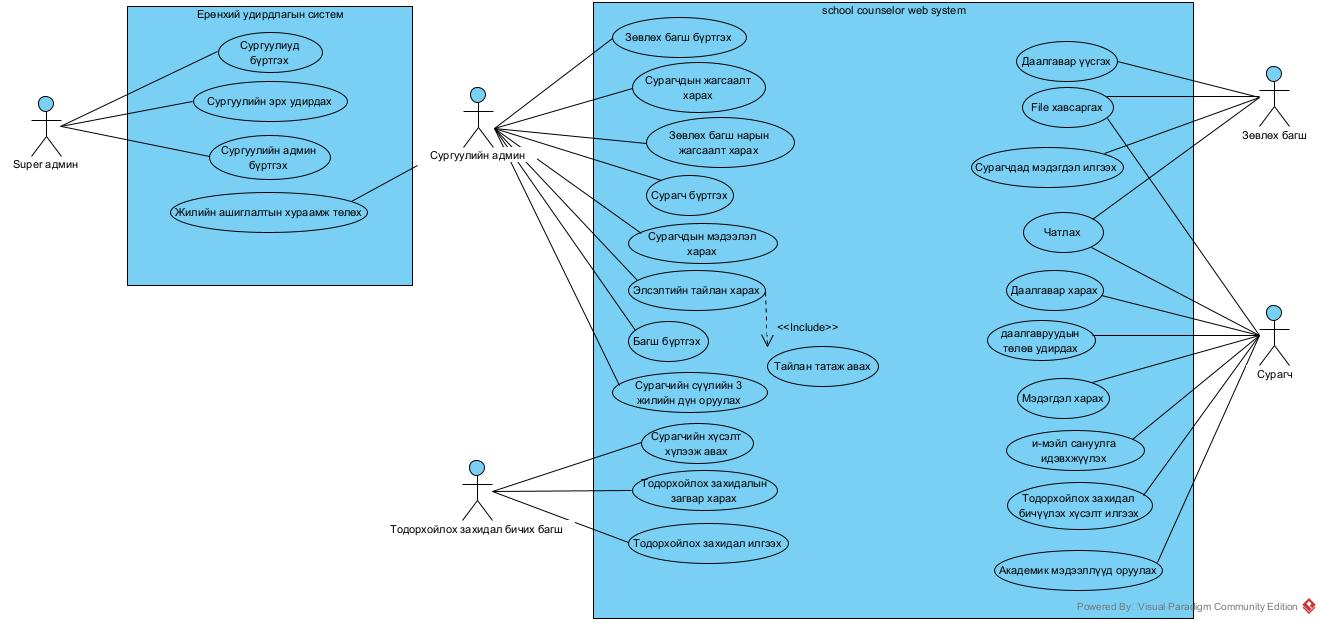
\includegraphics[scale=0.35]{Figures/chapter2/school counselor web system.jpg}
    \caption{Юзкейс диаграмм}
    \label{fig:usecase}
\end{figure}
\section{Юзкейсийн тодорхойлолт}

Энэхүү хэсэгт системийн үндсэн хэрэглэгчид болон
тэдгээрийн системтэй харилцах үйл ажиллагааг
юзкейсийн тодорхойлолтын аргаар дэлгэрэнгүй
тодорхойлсон. Юзкейс бүр нь хэрэглэгчийн зорилго,
системийн хариу үйлдэл болон мэдээллийн урсгалыг
дүрсэлнэ.

Системийн юзкейсүүд нь Супер админ, Сургуулийн
админ, Зөвлөх багш, Тодорхойлох захидал бичих
багш болон Сурагч гэсэн үндсэн хэрэглэгчдэд
хуваагдана.

Нийт 28 юзкейсын тодорхойлолтыг боловсруулсан
бөгөөд эдгээр нь системийн бүх үндсэн үйл
ажиллагааг хамарна.

\subsection*{Супер админы юзкейсүүд}

\begin{longtable}{|r|p{11cm}|}
\caption{Сургуулиуд бүртгэх}
\label{table:usecase1}\\ \hline
Юзкейс & Сургуулиуд бүртгэх \\ \hline
ID & 1 \\ \hline
Үндсэн тоглогч & Супер админ \\ \hline
Товч тайлбар & Супер админ систем ашиглах
сургуулийг платформд бүртгэнэ. \\ \hline
Өмнөх нөхцөл &
\begin{enumerate}[nosep]
\item Супер админ системд нэвтэрсэн байх.
\end{enumerate} \\ \hline
Үндсэн урсгал &
\begin{enumerate}[nosep]
\item Супер админ ``Сургууль бүртгэх'' хэсэгт орно.
\item Систем бүртгэлийн маягт харуулна.
\item Супер админ сургуулийн мэдээллийг оруулна.
\item ``Хадгалах'' товч дарна.
\item Систем мэдээллийг шалгана.
\item Хэрэв бүртгэл амжилттай бол:
\begin{enumerate}[nosep,label*=\arabic*.]
\item Систем сургуулийн бүртгэл үүсгэнэ.
\item Амжилттай тухай мэдэгдэл харуулна.
\end{enumerate}
\item Хэрэв бүртгэл амжилтгүй бол:
\begin{enumerate}[nosep,label*=\arabic*.]
\item Систем алдааны мэдэгдэл харуулна.
\end{enumerate}
\end{enumerate} \\ \hline
Дараах нөхцөл &
\begin{enumerate}[nosep]
\item Шинэ сургууль системд бүртгэгдсэн байх.
\end{enumerate} \\ \hline
\end{longtable}

\begin{longtable}{|r|p{11cm}|}
\caption{Сургуулийн эрх удирдах}
\label{table:usecase2}\\ \hline
Юзкейс & Сургуулийн эрх удирдах \\ \hline
ID & 2 \\ \hline
Үндсэн тоглогч & Супер админ \\ \hline
Товч тайлбар & Супер админ сургуулийн
систем ашиглах эрхийг идэвхжүүлэх болон
идэвхгүй болгоно. \\ \hline
Өмнөх нөхцөл &
\begin{enumerate}[nosep]
\item Супер админ системд нэвтэрсэн байх.
\item Сургууль системд бүртгэлтэй байх.
\end{enumerate} \\ \hline
Үндсэн урсгал &
\begin{enumerate}[nosep]
\item Супер админ сургуулиудын жагсаалт руу орно.
\item Тухайн сургуулийг сонгоно.
\item Систем дэлгэрэнгүй мэдээлэл харуулна.
\item Эрхийн төлөвийг өөрчилнө.
\item ``Хадгалах'' товч дарна.
\item Систем өөрчлөлтийг хадгална.
\item Амжилттай тухай мэдэгдэл харуулна.
\end{enumerate} \\ \hline
Дараах нөхцөл &
\begin{enumerate}[nosep]
\item Сургуулийн эрх шинэчлэгдсэн байх.
\end{enumerate} \\ \hline
\end{longtable}

\begin{longtable}{|r|p{11cm}|}
\caption{Сургуулийн админ бүртгэх}
\label{table:usecase3}\\ \hline
Юзкейс & Сургуулийн админ бүртгэх \\ \hline
ID & 3 \\ \hline
Үндсэн тоглогч & Супер админ \\ \hline
Товч тайлбар & Супер админ тухайн
сургуулийн админы бүртгэл үүсгэнэ. \\ \hline
Өмнөх нөхцөл &
\begin{enumerate}[nosep]
\item Супер админ системд нэвтэрсэн байх.
\item Сургууль бүртгэлтэй байх.
\end{enumerate} \\ \hline
Үндсэн урсгал &
\begin{enumerate}[nosep]
\item ``Админ бүртгэх'' хэсэгт орно.
\item Систем бүртгэлийн маягт харуулна.
\item Админы мэдээллийг оруулна.
\item ``Бүртгэх'' товч дарна.
\item Систем мэдээллийг шалгана.
\item Хэрэв амжилттай бол:
\begin{enumerate}[nosep,label*=\arabic*.]
\item Систем шинэ админы бүртгэл үүсгэнэ.
\item Амжилттай тухай мэдэгдэл харуулна.
\end{enumerate}
\item Хэрэв алдаа гарвал:
\begin{enumerate}[nosep,label*=\arabic*.]
\item Алдааны мэдэгдэл харуулна.
\end{enumerate}
\end{enumerate} \\ \hline
Дараах нөхцөл &
\begin{enumerate}[nosep]
\item Шинэ админ бүртгэгдсэн байх.
\end{enumerate} \\ \hline
\end{longtable}

\begin{longtable}{|r|p{11cm}|}
\caption{Жилийн ашиглалтын хураамж төлөх}
\label{table:usecase4}\\ \hline
Юзкейс & Жилийн ашиглалтын хураамж төлөх \\ \hline
ID & 4 \\ \hline
Үндсэн тоглогч & Супер админ \\ \hline
Товч тайлбар & Супер админ сургуулийн
жилийн хураамжийг QPay ашиглан баталгаажуулна.
\\ \hline
Өмнөх нөхцөл &
\begin{enumerate}[nosep]
\item Супер админ системд нэвтэрсэн байх.
\item Төлбөрийн хугацаа дууссан байх.
\end{enumerate} \\ \hline
Үндсэн урсгал &
\begin{enumerate}[nosep]
\item ``Төлбөр'' хэсэгт орно.
\item Систем төлбөрийн жагсаалт харуулна.
\item Төлбөрийг сонгоно.
\item Систем QPay callback шалгана.
\item Хэрэв төлбөр амжилттай бол:
\begin{enumerate}[nosep,label*=\arabic*.]
\item Систем эрх сунгана.
\item Төлбөрийн баримт үүсгэнэ.
\end{enumerate}
\item Хэрэв төлбөр амжилтгүй бол:
\begin{enumerate}[nosep,label*=\arabic*.]
\item Алдааны мэдэгдэл харуулна.
\end{enumerate}
\end{enumerate} \\ \hline
Дараах нөхцөл &
\begin{enumerate}[nosep]
\item Сургуулийн эрх сунгагдсан байх.
\end{enumerate} \\ \hline
\end{longtable}

\subsection*{Сургуулийн админы юзкейсүүд}

\begin{longtable}{|r|p{11cm}|}
\caption{Зөвлөх багш бүртгэх}
\label{table:usecase5}\\ \hline
Юзкейс & Зөвлөх багш бүртгэх \\ \hline
ID & 5 \\ \hline
Үндсэн тоглогч & Сургуулийн админ \\ \hline
Товч тайлбар & Сургуулийн админ шинэ
зөвлөх багшийн бүртгэл үүсгэнэ. \\ \hline
Өмнөх нөхцөл &
\begin{enumerate}[nosep]
\item Сургуулийн админ системд нэвтэрсэн байх.
\end{enumerate} \\ \hline
Үндсэн урсгал &
\begin{enumerate}[nosep]
\item ``Зөвлөх багш бүртгэх'' хэсэгт орно.
\item Систем бүртгэлийн маягт харуулна.
\item Багшийн мэдээллийг оруулна.
\item ``Бүртгэх'' товч дарна.
\item Систем мэдээллийг шалгана.
\item Хэрэв бүртгэл амжилттай бол:
\begin{enumerate}[nosep,label*=\arabic*.]
\item Систем бүртгэл үүсгэнэ.
\item Амжилттай тухай мэдэгдэл харуулна.
\end{enumerate}
\item Хэрэв алдаа гарвал:
\begin{enumerate}[nosep,label*=\arabic*.]
\item Алдааны мэдэгдэл харуулна.
\end{enumerate}
\end{enumerate} \\ \hline
Дараах нөхцөл &
\begin{enumerate}[nosep]
\item Зөвлөх багш бүртгэгдсэн байх.
\end{enumerate} \\ \hline
\end{longtable}

\begin{longtable}{|r|p{11cm}|}
\caption{Сурагчийн жагсаалт харах}
\label{table:usecase6}\\ \hline
Юзкейс & Сурагчийн жагсаалт харах \\ \hline
ID & 6 \\ \hline
Үндсэн тоглогч & Сургуулийн админ \\ \hline
Товч тайлбар & Системд бүртгэлтэй
сурагчдын жагсаалтыг харна. \\ \hline
Өмнөх нөхцөл &
\begin{enumerate}[nosep]
\item Сургуулийн админ нэвтэрсэн байх.
\end{enumerate} \\ \hline
Үндсэн урсгал &
\begin{enumerate}[nosep]
\item ``Сурагчид'' хэсэгт орно.
\item Систем сурагчдын жагсаалт харуулна.
\item Хайлт болон шүүлтүүр ашиглана.
\item Сурагч сонгоно.
\item Систем дэлгэрэнгүй мэдээлэл харуулна.
\end{enumerate} \\ \hline
Дараах нөхцөл &
\begin{enumerate}[nosep]
\item Сурагчдын мэдээлэл харагдсан байх.
\end{enumerate} \\ \hline
\end{longtable}

\begin{longtable}{|r|p{11cm}|}
\caption{Элсэлтийн тайлан харах}
\label{table:usecase12}\\ \hline
Юзкейс & Элсэлтийн тайлан харах \\ \hline
ID & 12 \\ \hline
Үндсэн тоглогч & Сургуулийн админ \\ \hline
Товч тайлбар & Сурагчдын элсэлтийн
статистик тайланг харна. \\ \hline
Өмнөх нөхцөл &
\begin{enumerate}[nosep]
\item Сургуулийн админ нэвтэрсэн байх.
\end{enumerate} \\ \hline
Үндсэн урсгал &
\begin{enumerate}[nosep]
\item ``Тайлан'' хэсэгт орно.
\item Систем статистик мэдээлэл харуулна.
\item Тайланг шүүнэ.
\item ``Татаж авах'' товч дарна.
\item Систем <<include>> харилцаагаар
``Тайлан татаж авах'' юзкейсыг дуудна.
\end{enumerate} \\ \hline
Дараах нөхцөл &
\begin{enumerate}[nosep]
\item Тайлан амжилттай харагдсан байх.
\end{enumerate} \\ \hline
\end{longtable}

\subsection*{Зөвлөх багшийн юзкейсүүд}

\begin{longtable}{|r|p{11cm}|}
\caption{Даалгавар үүсгэх}
\label{table:usecase19}\\ \hline
Юзкейс & Даалгавар үүсгэх \\ \hline
ID & 19 \\ \hline
Үндсэн тоглогч & Зөвлөх багш \\ \hline
Товч тайлбар & Зөвлөх багш ерөнхий
болон нэмэлт даалгавар үүсгэнэ. \\ \hline
Өмнөх нөхцөл &
\begin{enumerate}[nosep]
\item Зөвлөх багш нэвтэрсэн байх.
\end{enumerate} \\ \hline
Үндсэн урсгал &
\begin{enumerate}[nosep]
\item ``Даалгавар үүсгэх'' хэсэгт орно.
\item Систем маягт харуулна.
\item Даалгаврын мэдээлэл оруулна.
\item Сурагч сонгоно.
\item ``Хадгалах'' товч дарна.
\item Систем даалгавар үүсгэнэ.
\item Сурагчдад мэдэгдэл илгээнэ.
\end{enumerate} \\ \hline
Дараах нөхцөл &
\begin{enumerate}[nosep]
\item Даалгавар амжилттай үүссэн байх.
\end{enumerate} \\ \hline
\end{longtable}

\begin{longtable}{|r|p{11cm}|}
\caption{File хавсаргах}
\label{table:usecase20}\\ \hline
Юзкейс & File хавсаргах \\ \hline
ID & 20 \\ \hline
Үндсэн тоглогч & Зөвлөх багш \\ \hline
Товч тайлбар & Зөвлөмжийн материал
болон файл байршуулна. \\ \hline
Өмнөх нөхцөл &
\begin{enumerate}[nosep]
\item Зөвлөх багш нэвтэрсэн байх.
\end{enumerate} \\ \hline
Үндсэн урсгал &
\begin{enumerate}[nosep]
\item ``Файл хавсаргах'' хэсэгт орно.
\item Систем файл оруулах хэсэг харуулна.
\item Файл сонгож байршуулна.
\item Систем файл хадгална.
\item Сурагчдад харагдах байдлаар нийтэлнэ.
\end{enumerate} \\ \hline
Дараах нөхцөл &
\begin{enumerate}[nosep]
\item Файл системд хадгалагдсан байх.
\end{enumerate} \\ \hline
\end{longtable}

\subsection*{Сурагчийн юзкейсүүд}

\begin{longtable}{|r|p{11cm}|}
\caption{Чатлах}
\label{table:usecase22}\\ \hline
Юзкейс & Чатлах \\ \hline
ID & 22 \\ \hline
Үндсэн тоглогч & Сурагч \\ \hline
Нэмэлт тоглогч & Зөвлөх багш \\ \hline
Товч тайлбар & Сурагч зөвлөх багштай
бодит цагийн горимоор чатлана. \\ \hline
Өмнөх нөхцөл &
\begin{enumerate}[nosep]
\item Сурагч нэвтэрсэн байх.
\end{enumerate} \\ \hline
Үндсэн урсгал &
\begin{enumerate}[nosep]
\item ``Чат'' хэсэгт орно.
\item Систем чатын цонх харуулна.
\item Сурагч мессеж илгээнэ.
\item Зөвлөх багш хариу илгээнэ.
\item Систем мессежийг бодит цагт шинэчилнэ.
\end{enumerate} \\ \hline
Дараах нөхцөл &
\begin{enumerate}[nosep]
\item Чатын мэдээлэл хадгалагдсан байх.
\end{enumerate} \\ \hline
\end{longtable}

\begin{longtable}{|r|p{11cm}|}
\caption{Даалгавар харах}
\label{table:usecase23}\\ \hline
Юзкейс & Даалгавар харах \\ \hline
ID & 23 \\ \hline
Үндсэн тоглогч & Сурагч \\ \hline
Товч тайлбар & Өөрт оноогдсон
даалгавруудыг харна. \\ \hline
Өмнөх нөхцөл &
\begin{enumerate}[nosep]
\item Сурагч нэвтэрсэн байх.
\end{enumerate} \\ \hline
Үндсэн урсгал &
\begin{enumerate}[nosep]
\item ``Даалгавар'' хэсэгт орно.
\item Систем даалгаврын жагсаалт харуулна.
\item Сурагч даалгаврын мэдээллийг харна.
\end{enumerate} \\ \hline
Дараах нөхцөл &
\begin{enumerate}[nosep]
\item Даалгаврууд харагдсан байх.
\end{enumerate} \\ \hline
\end{longtable}

\begin{longtable}{|r|p{11cm}|}
\caption{Даалгаврын төлөв удирдах}
\label{table:usecase24}\\ \hline
Юзкейс & Даалгаврын төлөв удирдах \\ \hline
ID & 24 \\ \hline
Үндсэн тоглогч & Сурагч \\ \hline
Товч тайлбар & Даалгаврын гүйцэтгэлийн
түвшинг шинэчилнэ. \\ \hline
Өмнөх нөхцөл &
\begin{enumerate}[nosep]
\item Даалгавар оноогдсон байх.
\end{enumerate} \\ \hline
Үндсэн урсгал &
\begin{enumerate}[nosep]
\item Даалгавар сонгоно.
\item Систем дэлгэрэнгүй мэдээлэл харуулна.
\item Гүйцэтгэлийн түвшин оруулна.
\item ``Хадгалах'' товч дарна.
\item Систем төлөв шинэчилнэ.
\end{enumerate} \\ \hline
Дараах нөхцөл &
\begin{enumerate}[nosep]
\item Даалгаврын төлөв шинэчлэгдсэн байх.
\end{enumerate} \\ \hline
\end{longtable}

\begin{longtable}{|r|p{11cm}|}
\caption{Мэдэгдэл харах}
\label{table:usecase25}\\ \hline
Юзкейс & Мэдэгдэл харах \\ \hline
ID & 25 \\ \hline
Үндсэн тоглогч & Сурагч \\ \hline
Товч тайлбар & Ирсэн мэдэгдлүүдийг харна.
\\ \hline
Өмнөх нөхцөл &
\begin{enumerate}[nosep]
\item Сурагч нэвтэрсэн байх.
\end{enumerate} \\ \hline
Үндсэн урсгал &
\begin{enumerate}[nosep]
\item ``Мэдэгдэл'' хэсэгт орно.
\item Систем мэдэгдлийн жагсаалт харуулна.
\item Мэдэгдэл сонгон дэлгэрэнгүйг харна.
\end{enumerate} \\ \hline
Дараах нөхцөл &
\begin{enumerate}[nosep]
\item Мэдэгдэл амжилттай харагдсан байх.
\end{enumerate} \\ \hline
\end{longtable}

\begin{longtable}{|r|p{11cm}|}
\caption{И-мэйл сануулга идэвхжүүлэх}
\label{table:usecase26}\\ \hline
Юзкейс & И-мэйл сануулга идэвхжүүлэх \\ \hline
ID & 26 \\ \hline
Үндсэн тоглогч & Сурагч \\ \hline
Товч тайлбар & Даалгаврын хугацааны
сануулга и-мэйлээр авах тохиргоо хийнэ.
\\ \hline
Өмнөх нөхцөл &
\begin{enumerate}[nosep]
\item Сурагч нэвтэрсэн байх.
\end{enumerate} \\ \hline
Үндсэн урсгал &
\begin{enumerate}[nosep]
\item ``Тохиргоо'' хэсэгт орно.
\item Систем тохиргоо харуулна.
\item Сануулгыг идэвхжүүлнэ.
\item Систем тохиргоог хадгална.
\item Даалгаврын хугацаа дөхөх үед
автоматаар и-мэйл илгээнэ.
\end{enumerate} \\ \hline
Дараах нөхцөл &
\begin{enumerate}[nosep]
\item И-мэйл сануулга идэвхжсэн байх.
\end{enumerate} \\ \hline
\end{longtable}

\begin{longtable}{|r|p{11cm}|}
\caption{Академик мэдээлэл оруулах}
\label{table:usecase28}\\ \hline
Юзкейс & Академик мэдээлэл оруулах \\ \hline
ID & 28 \\ \hline
Үндсэн тоглогч & Сурагч \\ \hline
Товч тайлбар & GPA, шалгалтын оноо,
гадуурх үйл ажиллагаа болон сонирхсон
сургуулийн мэдээллийг оруулна. \\ \hline
Өмнөх нөхцөл &
\begin{enumerate}[nosep]
\item Сурагч системд нэвтэрсэн байх.
\end{enumerate} \\ \hline
Үндсэн урсгал &
\begin{enumerate}[nosep]
\item ``Профайл'' хэсэгт орно.
\item Систем мэдээлэл оруулах маягт харуулна.
\item Академик мэдээллээ оруулна.
\item ``Хадгалах'' товч дарна.
\item Систем мэдээллийг хадгална.
\item AI модуль мэдээлэл боловсруулна.
\item ``Safety'', ``Match'', ``Reach''
ангиллаар сургуулийн зөвлөмж гаргана.
\end{enumerate} \\ \hline
Дараах нөхцөл &
\begin{enumerate}[nosep]
\item AI зөвлөмж амжилттай гарсан байх.
\end{enumerate} \\ \hline
\end{longtable}
\section{Шинжилгээний класс диаграмм}
\paragraph{} Зураг \ref{fig:sh-class} Зураг 2.2 дээрх шинжилгээний класс диаграмм нь системийн гол элементүүд болох
классуудыг, тэдгээрийн шинж чанар, функц мөн холбоо хамаарал болон мэдээллийн
урсгалыг дүрсэлснийг харуулж байна. Энэ диаграмм нь системийн үндсэн өгөгдлүүд
хэрхэн хадгалагдах, боловсруулагдах болон классууд хоорондоо хэрхэн харилцан
ажиллаж байгааг тодорхойлно.

Диаграммд User, Student, Counselor, SchoolAdmin, SuperAdmin, Task, File,
Notification, Chat, AcademicInfo, Payment зэрэг үндсэн классууд багтсан.
Эдгээр классуудын хоорондын холбоо нь системийн хэрэглэгчид, даалгавар,
мэдэгдэл, файл болон академик мэдээллийн урсгалыг дүрсэлж байна.

Мөн Student класс нь Task, File, Chat, AcademicInfo зэрэг классуудтай
холбогдсоноор сурагчийн даалгаврын удирдлага, файл хадгалалт, чат харилцаа
болон академик мэдээллийг нэгтгэн удирдах боломжийг бүрдүүлж байна.
Counselor класс нь даалгавар үүсгэх, мэдэгдэл илгээх, сурагчтай чатлах зэрэг
үйл ажиллагаатай холбогдсон бол SchoolAdmin болон SuperAdmin классууд нь
сургуулийн удирдлага, хэрэглэгчийн эрхийн зохицуулалт болон subscription
удирдлагыг хэрэгжүүлнэ.

Түүнчлэн Payment класс нь сургуулийн төлбөрийн мэдээллийг хадгалах,
Notification класс нь системийн мэдэгдлийг хэрэглэгчид хүргэх, Chat класс нь
хэрэглэгчдийн хоорондын бодит цагийн харилцааг дэмжих зориулалттайгаар
тус тус тодорхойлогдсон.

Энэхүү диаграмм нь системийн бүтэц, мэдээллийн уялдаа холбоо болон
үндсэн үйл ажиллагааны логикийг ойлгоход чухал үүрэгтэй.

\begin{figure}[H]
    \centering
    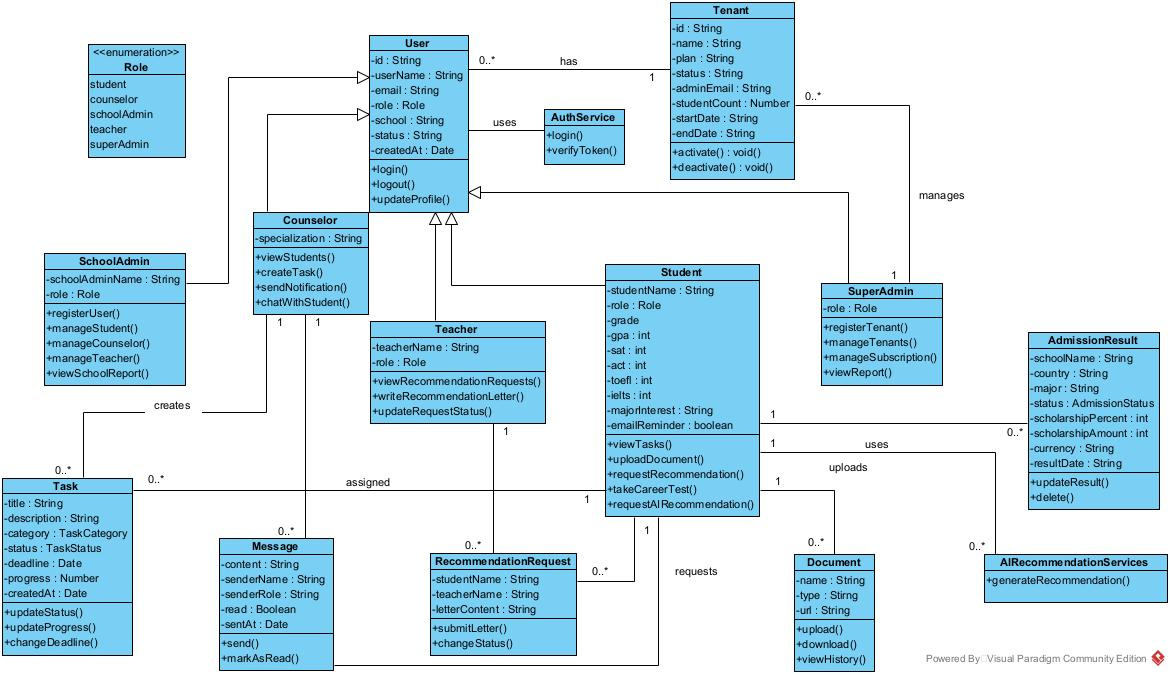
\includegraphics[scale=0.4]{Figures/chapter2/designclass.jpg}
    \caption{Шинжилгээний класс диаграмм}
    \label{fig:sh-class}
\end{figure}




\section{Үйл ажиллагааны диаграмм}
\paragraph{}
Ахлах сургуулийн зөвлөгчийн веб системийн юзкейс диаграммд тодорхойлогдсон
юзкейсүүдийн эхлэлээс төгсгөл хүртэлх үйлдлүүдийг дүрсэлсэн
үйл ажиллагааны диаграммыг доор харуулав.
\par \noindent
Хэрэглэгч зөвлөгчийн веб системийг ашиглахын тулд эхлээд
бүртгэлтэй эсэхээ шалгуулна. Хэрэв бүртгэлтэй бол нэвтрэх
хэсгээр дамжин системд нэвтэрч, өөрийн эрхийн дагуу үйл
ажиллагаа гүйцэтгэнэ. Харин бүртгэлгүй хэрэглэгч бүртгэлийн
форм бөглөж, и-мэйл баталгаажуулалтын дараа бүртгэл үүсгэнэ.

Сурагч нь академик мэдээллээ оруулах, AI зөвлөмж авах,
даалгавар харах болон даалгаврын төлөв шинэчлэх
боломжтой. Зөвлөх багш нь сурагчдад даалгавар үүсгэх,
файл хавсаргах, мэдэгдэл илгээх болон чатлах үйл ажиллагаа
гүйцэтгэнэ. Мөн сургуулийн админ, тодорхойлох захидал
бичих багш болон супер админ нь өөрсдийн эрхийн хүрээнд
холбогдох үйл ажиллагаануудыг гүйцэтгэнэ.

Үйл ажиллагааны төгсгөлд өгөгдөл хадгалагдаж, хэрэглэгчид
тухайн үйлдлийн үр дүн харагдана. Дээрх процессыг
Зураг \ref{fig:activity-counselor}-ийн зөвлөгчийн веб системийн
нэгдсэн үйл ажиллагааны диаграммаас харж болно.
\begin{figure}[H]
    \centering
    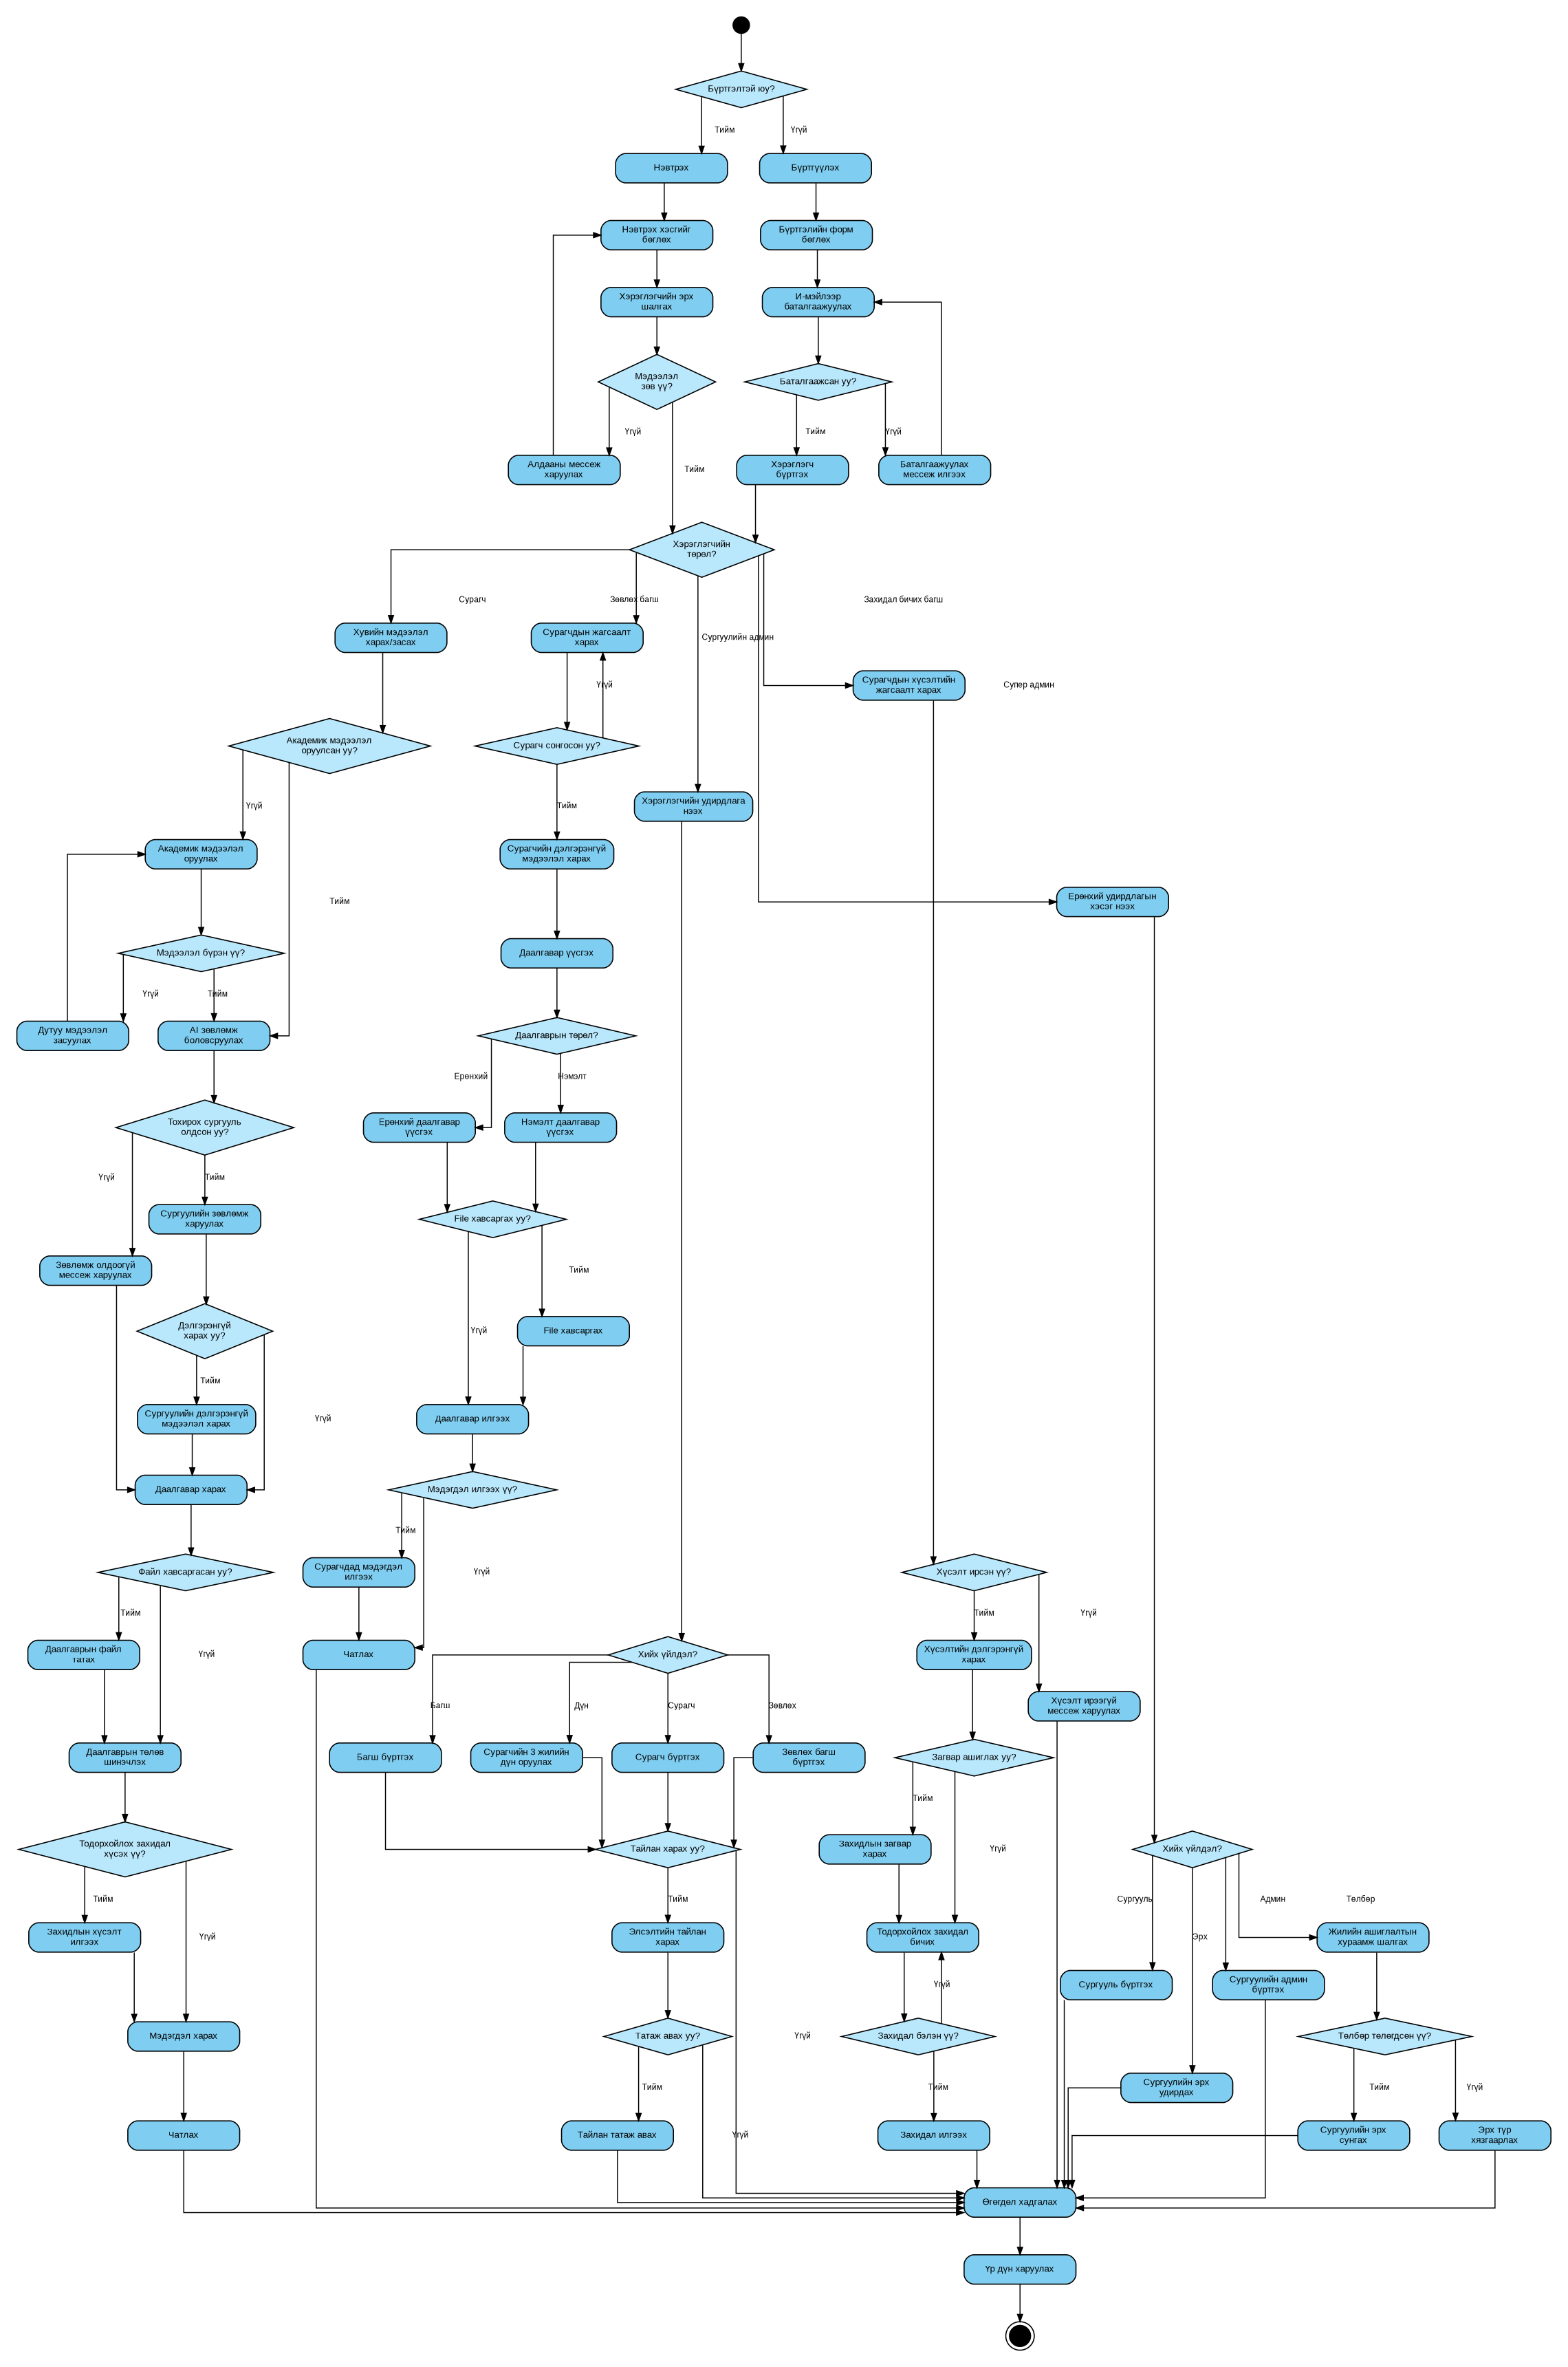
\includegraphics[scale=0.2]{Figures/chapter2/activity.png}
    \caption{Үйл ажиллагааны диаграмм}
    \label{fig:activity-counselor}
    \label{fig:ua-burtgel-zh}
\end{figure}
\par \noindent

\section{Бүлгийн дүгнэлт}
\paragraph{} Энэхүү бүлэгт зөвлөгчийн веб системийн функциональ болон
функциональ бус шаардлагуудыг тодорхойлж, хэрэглэгчдийн
хэрэгцээнд тулгуурласан системийн шинжилгээг хийлээ.
Мөн сурагч, зөвлөх багш, сургуулийн админ, тодорхойлох
захидал бичих багш болон супер админ гэсэн үндсэн
оролцогчдын үүрэг, боломжуудыг тодорхойлон юзкейс
диаграмм болон юзкейсийн тодорхойлолтуудыг боловсруулсан.

Системийн үндсэн үйл ажиллагаанууд болох бүртгүүлэх,
нэвтрэх, академик мэдээлэл оруулах, AI зөвлөмж авах,
даалгавар удирдах, файл хавсаргах, мэдэгдэл илгээх,
чатлах болон тодорхойлох захидлын хүсэлт илгээх зэрэг
процессуудыг шинжилгээний түвшинд тодорхойлсон.
Үүний зэрэгцээ системийн өгөгдлийн урсгал болон
объектуудын хамаарлыг шинжилгээний класс диаграмм
болон үйл ажиллагааны диаграммаар дүрсэлсэн.

Ингэснээр системийн бүтэц, өгөгдлийн холбоо хамаарал,
хэрэглэгчдийн оролцоо болон үндсэн үйл ажиллагааны
урсгал тодорхой болсон.
